%\documentclass[journal]{vgtc}                % final (journal style)
\documentclass[review,journal]{vgtc}         % review (journal style)
%\documentclass[widereview]{vgtc}             % wide-spaced review
%\documentclass[preprint,journal]{vgtc}       % preprint (journal style)
%\documentclass[electronic,journal]{vgtc}     % electronic version, journal

%% Uncomment one of the lines above depending on where your paper is
%% in the conference process. ``review'' and ``widereview'' are for review
%% submission, ``preprint'' is for pre-publication, and the final version
%% doesn't use a specific qualifier. Further, ``electronic'' includes
%% hyperreferences for more convenient online viewing.

%% Please use one of the ``review'' options in combination with the
%% assigned online id (see below) ONLY if your paper uses a double blind
%% review process. Some conferences, like IEEE Vis and InfoVis, have NOT
%% in the past.

%% Please note that the use of figures other than the optional teaser is
%% not permitted on the first page of the journal version.  Figures should
%% begin on the second page and be in CMYK or Grey scale format,
%% otherwise, colour shifting may occur during the printing process.
%% Papers submitted with figures other than the optional teaser on the
%% first page will be refused.

%% These three lines bring in essential packages: ``mathptmx'' for Type 1
%% typefaces, ``graphicx'' for inclusion of EPS figures. and ``times''
%% for proper handling of the times font family.
\usepackage{mathptmx}
\usepackage{graphicx}
\usepackage{epstopdf}
\usepackage{times}

%% We encourage the use of mathptmx for consistent usage of times font
%% throughout the proceedings. However, if you encounter conflicts
%% with other math-related packages, you may want to disable it.

%% This turns references into clickable hyperlinks.
\usepackage[bookmarks,backref=true,linkcolor=black]{hyperref} %,colorlinks
\hypersetup{
  pdfauthor = {},
  pdftitle = {},
  pdfsubject = {},
  pdfkeywords = {},
  colorlinks=true,
  linkcolor= black,
  citecolor= black,
  pageanchor=true,
  urlcolor = black,
  plainpages = false,
  linktocpage
}

% Select what to do with command \comment:
\newcommand{\comment}[1]{}  %comment not showed
%\newcommand{\comment}[1]
%{\par {\bfseries \color{blue} #1 \par}} %comment showed
%% If you are submitting a paper to a conference for review with a double
%% blind reviewing process, please replace the value ``0'' below with your
%% OnlineID. Otherwise, you may safely leave it at ``0''.
\onlineid{0}

%% declare the category of your paper, only shown in review mode
\vgtccategory{Research}

%% allow for this line if you want the electronic option to work properly
\vgtcinsertpkg

%% In preprint mode you may define your own headline.
%\preprinttext{To appear in IEEE Transactions on Visualization and Computer Graphics.}

%% Paper title.

\title{InterventionViz: Visual Analysis of Behavior-Change Intervention Dynamics}

%% This is how authors are specified in the journal style

%% indicate IEEE Member or Student Member in form indicated below
\author{T. Murray \textit{Student Member, IEEE}, D. Spruijt-Metz, E. Hekler, A. Raij \textit{Member, IEEE}}
\authorfooter{
%% insert punctuation at end of each item
\item
 T. Murray is with the University of South Florida. E-mail: tylarmurray@mail.usf.edu.
\item
 D. Spruijt-Metz is with the Univeristy of Southern California Center for Economic and Social Research.
\item
 E. Hekler is with Arizona State University.
\item
 A. Raij is with the University of Central Florida Institute for Simulation and Training.
}

%other entries to be set up for journal
\shortauthortitle{Biv \MakeLowercase{\textit{et al.}}: InterventionViz}
%\shortauthortitle{Firstauthor \MakeLowercase{\textit{et al.}}: Paper Title}

%% Abstract section.
\abstract{
With the advent of research-grade wearable sensor suites and increasingly ubiquitous human-computer interface comes the opportunity for a new generation of behavioral theory and behavior change methodologies.
Just-in-time interventions (JITIs) designed to optimize a subjects behavior based on their momentary context are under exploration as a potentially powerful ally for practitioners and commercial behavior health applications.
Analysis of the effect an intervention has on a target behavior, however, is a complex task not well handled by current methods.

In this work we explore the application of aggregated time-series visualization techniques to aid analysis of intervention event effects with emphasis on the dynamics of participant response to intervention.
To highlight the strengths and caveats of the techniques employed, data from two trial studies of physical activity interventions (n=11, n=10) and one empirical control dataset (n=1) are utilized.
The insights presented in this work offer a foundation for future visualization research addressing this problem and as a guide for behavioral scientists in need of more novel methods of analysis.
} % end abstract

%% Keywords that describe your work. Will show as 'Index Terms' in journal
%% please capitalize first letter and insert punctuation after last keyword
\keywords{Visualization in Social and Information Sciences, Hypothesis Testing, Visual Evidence, Time Series Data, Qualitative Evaluation, Biomedical and Medical Visualization}

%% ACM Computing Classification System (CCS).
%% See <http://www.acm.org/class/1998/> for details.
%% The ``\CCScat'' command takes four arguments.

\CCScatlist{ % not used in journal version
 \CCScat{J.4.1}{Computer Applications}{Social and Behavioral Sciences}{Psychology};
 \CCScat{I.6.5}{Computing Methodologies}{Simulation and Modeling}{Model Development}
}

%% Uncomment below to include a teaser figure.
  \teaser{
   \centering
   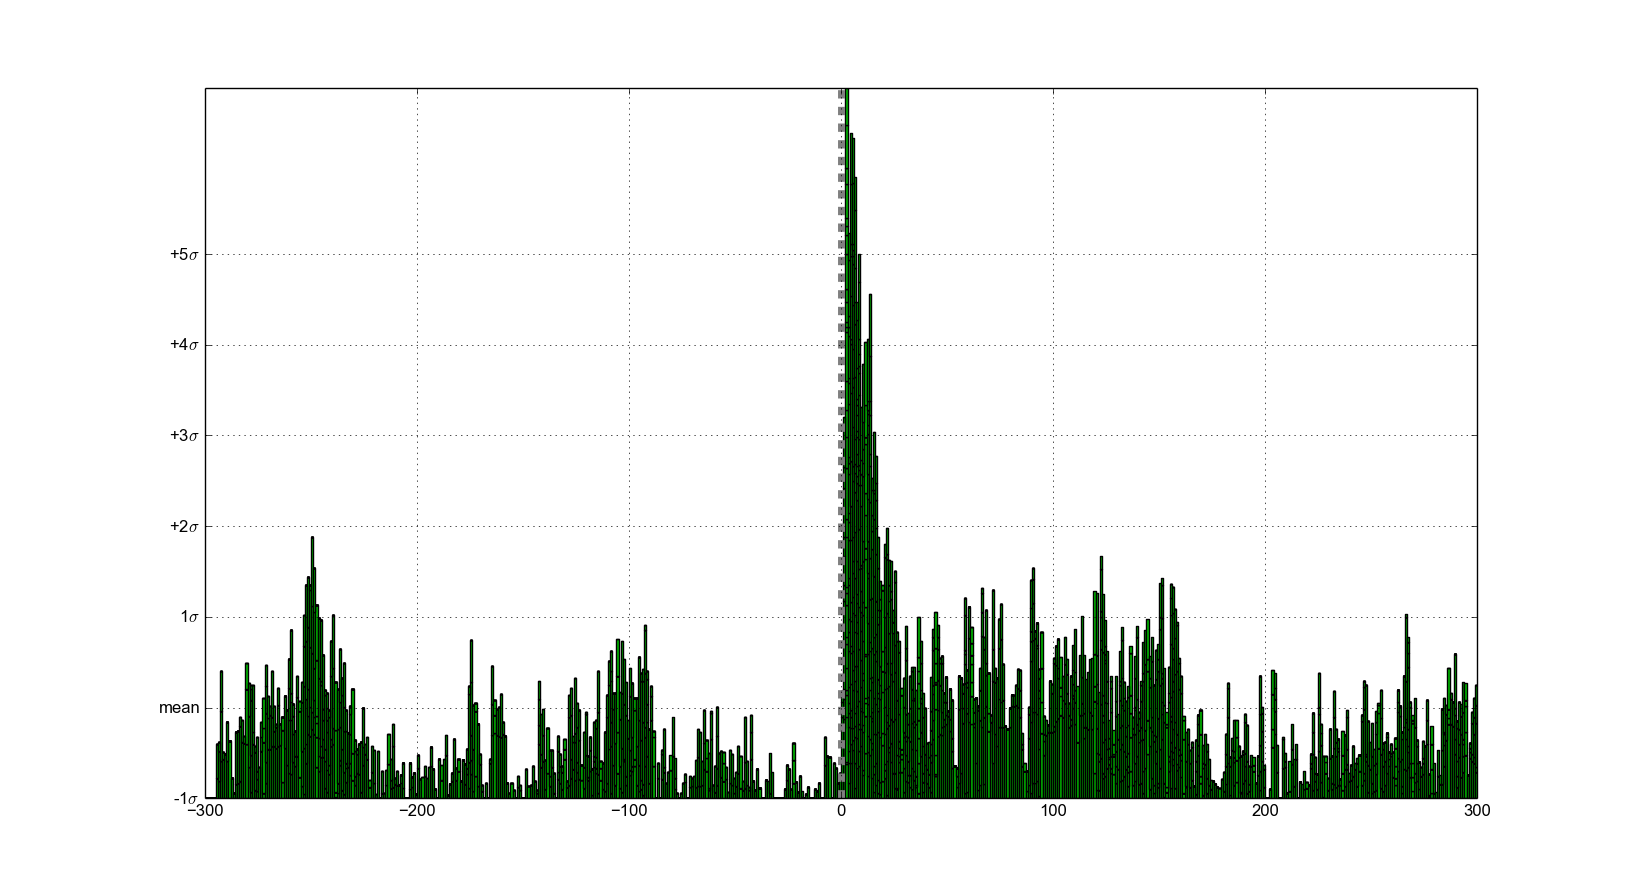
\includegraphics[width=16cm]{./img/teaser}
   
   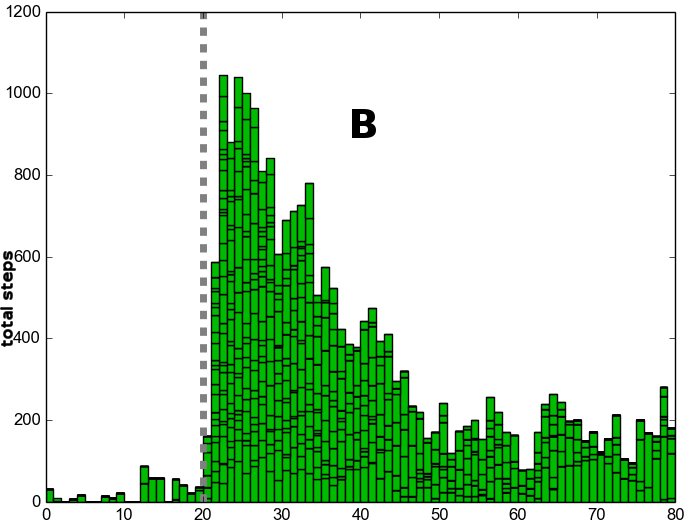
\includegraphics[width=5cm]{./img/teaser/perfect_intervention_stack.png}
   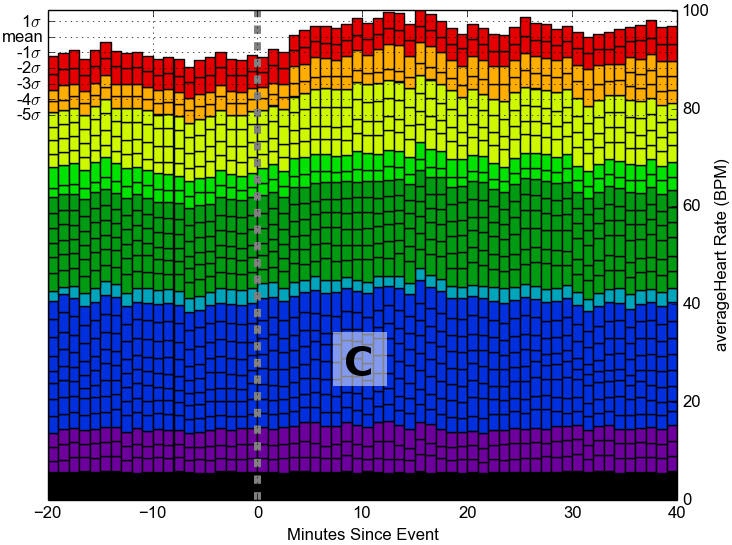
\includegraphics[width=5cm]{./img/teaser/knowMe_60m_bars.png}
   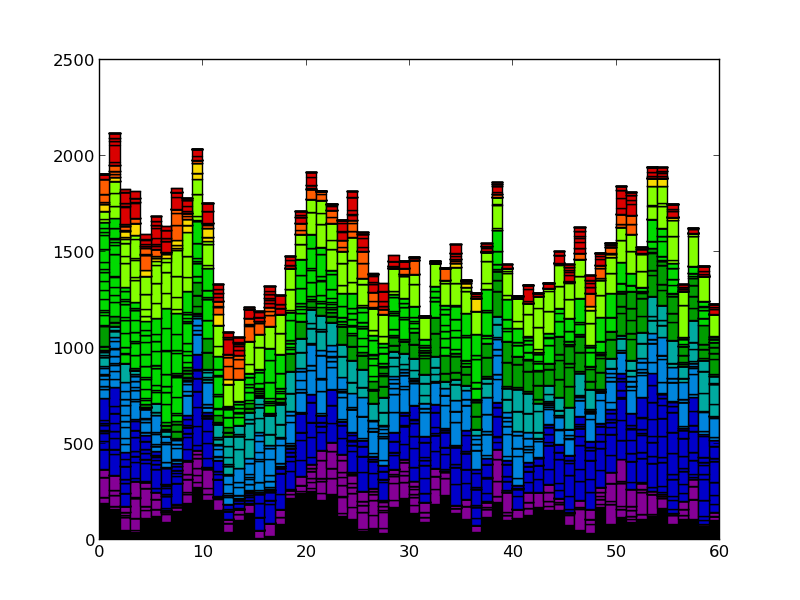
\includegraphics[width=5cm]{./img/teaser/steps_60m_after_view_event_active.png}
   
   \caption{
    A)Aggregated step counts surrounding an intervention event shows event response dynamics and individual variations across events. 
    B) Aggregation of step counts showing dramatic response to the the control intervention. 
    C) Heart rate data aggregated across KnowMe particpants shows a mild response to an SMS intervention. 
    D) Aggregated step counts of subjects briefly exposed to an active mAvatar shows little trend. 
   }
  }

%% Uncomment below to disable the manuscript note
%\renewcommand{\manuscriptnotetxt}{}

%% Copyright space is enabled by default as required by guidelines.
%% It is disabled by the 'review' option or via the following command:
% \nocopyrightspace

%%%%%%%%%%%%%%%%%%%%%%%%%%%%%%%%%%%%%%%%%%%%%%%%%%%%%%%%%%%%%%%%
%%%%%%%%%%%%%%%%%%%%%% START OF THE PAPER %%%%%%%%%%%%%%%%%%%%%%
%%%%%%%%%%%%%%%%%%%%%%%%%%%%%%%%%%%%%%%%%%%%%%%%%%%%%%%%%%%%%%%%%

\begin{document}

%% The ``\maketitle'' command must be the first command after the
%% ``\begin{document}'' command. It prepares and prints the title block.

%% the only exception to this rule is the \firstsection command

%% \firstsection{Introduction}

\maketitle


\section{Introduction} %for journal use above \firstsection{..} instead


% integrate and expand
\comment{






To be effective, such tools should have several characteristics.
}


Health sensing, machine learning, network access, and computation are rapidly becoming ubiquitous, enabling new tools for capturing human activities in the natural environment, often at very small time scales.  Previous work shows such tools can be used to detect behaviors and psychological states such as stress\cite{chang2011,lu2012}, physical activity\cite{li2010,emken2012}, social interaction\cite{wyatt2011}, and smoking\cite{sazonov2011}, automatically and, in some cases, in real-time. Likewise, there are many commercial, inexpensive, consumer-grade products (Jawbone Up, Fitbit, Nike Plus to name a few) that are putting these data in the hands of the layperson. The challenge that both laypeople and health research communities face is in making sense of this data.

Health researchers - and by extension overall public health - could benefit significantly from access to tools that make sense of these data.    Many of today's greatest health challenges can be mapped back to  behavioral choices made in-the-moment as people go about normal daily life.  Avoiding physical activity, eating high-fat foods, and smoking cigarettes are all poor behavioral choices made in-the-moment that, in aggreggate, lead to a variety of health problems (e.g., obesity, diabetes, heart disease, cancer, chronic pain, depression), lower quality of life and shortened lifespans \cite{franco2005, dunn2001, yanbaeva2007, ross2000}.  Unfortunately, the tools health researchers need do not yet exist to manage, review, and learn from such data.  Information visualization can play a role in enabling such tools.

With the right tools \cite{}, health researchers could better examine important behavioral events and coexisting contextual factors at a level of detail and richness not previously possible.

Likewise, they can go beyond observing events.  They could deliver interventions to individuals in-the-moment, and then see how the intervention in turn changes behavior and affect.


v


Of particular interest to the health research research community is the concept of the just-in-tim


These data provide new opportunities for the human-computer interaction (HCI), behavioral science, and other related communities to develop user interfaces for mobile behavioral interventions that help users make better in the moment behavioral choices related to health\cite{klasnja2012,nahum2012}, productivity\cite{ho2005,sohn2005,jewell2011}

New methods for evaluating these behavioral interventions remain underexplored and conventional methods of analysis do not offer the level of detail needed to explore the implicit dynamics of just-in-time, interactive, or adaptive interventions.


In addition to metrics of success of an intervention, behavioral theorists need tools to help understand the dynamics of behavioral responses to a stimulus.
Due to the lack of a dynamical treatment of behavior within theories, existing models behavior appear inadequate to inform state-of-the-art intervention development \cite{riley2011}.
Applicable methods of intervention analysis and data visualization have been slow to reach behavioral researchers, dramatically limiting their ability to develop of state-of-the-art behavioral theories to address these shortcomings.


% This paragraph discusses our workflow.  What did we do - step by step - to produce our contributions and reach our conclusions?
In this paper, we derive visualizations that help behavioral scientists gain insight into the short time scale dynamics of health-related events. We focus specifically on the needs of behavioral scientists because many have access to such event datasets but do not yet have the tools to better understand health events, derive and test behavioral theories from them, and ultimately develop more effective and usable behavioral health interventions. The work can be divided into three stages.

\textit{First}, we conduct a user needs analysis with a vested group of stakeholders. We held a data-gathering session at a top-tier behavioral science conference as well as interacted informally with behavioral scientists with specific experience and goals of capturing, analyzing and learning from pervasive health data. We also collected  and analyzed event datasets with short-time scales generated by behavioral scientists. From these interactions and data, we define a set of user goals and tasks as well as broader design considerations for behavioral health event dynamics.

\textit{Second}, based on lessons learned from the user needs analysis, we design visualizations and demonstrate them on three datasets, each of which shows the effect of a physical activity intervention on a user. Two of the datasets were captured from children (ages 11 - ???) as they went about normal daily life, over a multi-day period (3 - 8 days).  The third dataset is a control dataset that mimics the ideal response to a "perfect" physical activity intervention.

\textit{Third}, we derive lessons learned from the proposed visualizations, focusing on 1) what the visualizations do and do not reveal about the data, 2) where there is uncertainty in the meaning of the visualizations, and 3) what scientific questions are not answered by these visualizations and thus require future work.

% This paragraph summarizes contributions and conclusions from the above work. % Bulleted list of 2-3 contributions
These efforts led to the following important contributions to both the fields of behavioral science and information visualization.

\begin{enumerate}
	\item{a set of design considerations to guide visualization and tool design in this domain}
	\item{introduction to intervention response dynamics in relation to developing theories}
	\item{visualization methods which address some key tasks addressing the goals identified in the design considerations section}
\end{enumerate}

Ultimately, we conclude that ... % could just save this for the end...don't want to give away everything do we?

\comment{

%much of this will be re-integrated

Despite significant advances in the theory and practice of behavioral science, humans continue make poor behavioral choices on a daily basis, and the reasons for those choices remain, to some extent, uncharted.
The consequences of these daily choices are often insignificant in the moment but over time build up to larger individual and societal problems.


Similar challenges exist outside the realm of personal health.
Academic success is a function of attending class and completing assigned tasks, among other daily behaviors\cite{cooper2006}.
In personal finance, poor day-to-day purchasing decisions can add up to large financial debts\cite{norvilitis2003}.



\subsubsection{Contributions}
% summarize previous work (1 paragraph)


% summarize work done (1 paragraph - maybe a long one)
}

% an alternative framing of of our contributions:
\comment{
	- to understand how we can use this type of data to accomplish these domain-specific tasks?
	- to propose new hypotheses and techniques to support these tasks?
	- to propose lessons learned that may apply for similar viz problems.


% highlight why should viz community care!
This work breaks new ground in the application domain, but also provides guidelines for future work bridging the data visualization and behavioral science communities.
}

\section{Previous Work}

\subsection{Related Event-based Time Series Visualization}
"Lifelines" \cite{plaisant1996} allow for the exploration of events in a series for one individual, and new research in event sequence analysis \cite{Wongsuphasawat2011}, including analysis of event patterns \cite{Wongsuphasawat2012, fails2006, vrotsou2007} and the relation of multiple symptoms \cite{wongsuphasawat2011outflow} helps researchers examine outcomes on a "macro-scale" across many subjects by aggregating records into a single view.
Additionally, the problem of identifying patterns at multiple time scales has been partially addressed through clustering of time series \cite{van1999}, and methods for exploring the "paths" traversed by many individuals between many event types and statistical analyses to highlight relationships between events has recently been established \cite{gotz2014}.

Little existing work addresses the dynamics of a numerical variable's response to a behavioral intervention event.
Statistical methods of intervention analysis \cite{box1975}, have been applied across various disciplines but thus far there has been little demand for these methods in behavioral science.
Only recently has new wearable sensing technology made time-intensive, in-the-wild measurements feasible.
Additionally, the prospect of ubiquitous intervention delivery via mobile devices and the concept of Just-in-Time-Adaptive-Interventions (JiTAIs) have introduced a new demand for a more detailed understanding of human behavior.

\subsection{Current Intervention Methods}
Recent advances in sensing and ubiquitous computing have enabled examination of and influence over behavior at relatively high frequency (on the order of seconds) and in a wide range of daily life contexts.
New wearable sensing technologies are changing the way researchers do experiments, and mobile phones are a powerful new medium for delivering behavioral interventions "just-in-time".

Recent works have explored "adaptive interventions" tailored based on "tailoring variables" which may include user preferences, context, and personality \cite{collins2004}.
Despite these drastic changes in the interventions, methods for evaluating adaptive interventions remain in many ways similar to "fixed" interventions \cite{collins2004}, and the use of the multiphase optimization strategy (MOST) and sequential multiple assignment randomized trials (SMART) \cite{collins2007} maximize efficiency in applying these methods.
These methods become more difficult to apply, however, when dealing with Just in Time Adaptive Interventions (JiTAIs) \cite{nahum2014just}.

Existing work on visual analysis of systems usability \cite{harrison1994} may be applied to the evaluation of JiTAI systems, however, these methods focus largely on a single record, rather than generalizations drawn from across many.
Additionally, little theoretical guidance in terms of effect latency or delay exists to aid in the planning or analysis of experimental trials.

A theoretical basis which takes dynamical effects into consideration to enable improved behavioral intervention optimization has been proposed for interventions mediating gestational weight gain \cite{dong2013}, smoking behavior \cite{timms2014}, childhood anxiety \cite{pina2014}, and fibromyalgia \cite{deshpande2014}.
This new type of theoretical model is most effective on the timescale of multiple days, weeks, or months - partially because the confounds of contextual, within-day variations make analysis at this level difficult, but mostly because theories of behavior at this time scale are underdeveloped.
Methods for analyzing the dynamics of intervention responses using existing data are needed in order to catalyze the development of theories to explain these signals.

\section{Design Considerations}
%  How is the problem here similar to what has come before?
Many of the research questions faced by JiTAI developers are similar to those of fixed interventions. 
Researchers primary concerns remain centered around assessment of an intervention's ability to effect the target behavior.
Assessments are similarly judged by their reliability and validity, and good study design remains central to a good validation of intervention efficacy.

% How is it different?  
In addition to those existing, new challenges unique to JiTAI design and analysis must be addressed.
As interventions grow in their abilities to adapt, the search space of the problem grows exponentially.
Each additional "tailoring variable" or parameter added causes combinatorial increases, eventually making strictly empirical methods unfeasible.
In order to generalize existing experimental results to provide guidance, researchers typically turn to theory, however, theoretical models of behavior at the small timescales applicable to JiTAIs are underdeveloped and largely unsupported by empirical data. 
Though research questions remain the same, the additional challenges introduced in JiTAI design suggest that more detailed analysis and more rigorous modeling methods may be appropriate.
In addition to guiding the design of JiTAIs, quantitative modeling of behavior response over time would allow for JiTAIs to optimize interventions based on context-aware, personalized models.
%In order to enable development of these models, data visualization methods for exploring intervention effect over time and across participants are needed. 

When asked about the biggest hurdle blocking simulation and modeling from breaking into behavioral science, a majority of responders cited the need for better tools and collaboration to improve their understanding of the techniques.
In order to facilitate development of these tools and spur exploration of dynamical models of human behavior, we present a set of design considerations which have been developed through close collaboration with domain experts in JiTAI development.
These considerations include a listing of some common goals of a contemporary intervention researcher and a description of the typical characteristics of intervention datasets. 

\subsection{User Goals}
In this section we define the primary goals of a behavior-change intervention researcher looking to apply JiTAIs.
These goals have been developed through an extensive literature review, a survey of 11 behavioral scientists interested in applying modeling and simulation to their work, and close collaboration with domain experts.

\subsubsection{Assess Intervention Effectiveness}
%(efficacy,
First and foremost researchers are interested in showing that their intervention was effective.
T-tests and p-values - despite their shortcomings \cite{nuzzo2014} - have long dominated this domain, so researchers are looking for equally succinct indicators of success.
The nature of highly-personalized, context-dependent, and rapidly-optimized JiTAIs makes these analyses difficult for specific subsets of interventions, and thus researchers have been limited to testing entire systems over larger time-scales - comparing intervention-on vs control days, for instance.

\subsubsection{Response and Effectiveness vs Subgroups}
For most researchers it is not enough just to confirm efficacy of an intervention system, a closely tied second goal of the behavioral researcher is to characterize how the intervention works.
One way the behavioral researcher explores how an intervention works is to characterize how differences among individuals, sub-groups, and contexts affect effectiveness and characteristics of the response.
Subgroup analysis allows for existing theories to grow in complexity through incorporation of new conditions.
Particularly in the case of JiTAIs, a wide range of intervention types can be delivered and analysis of the efficacy of these different types in different contexts or applied to different subgroups has great potential to inform behavioral theory.


\subsubsection{Characterize Intervention Response}
Multiple behavioral intervention reviews have shown that interventions explicitly based on psychological theory are more effective \cite{glanz2010}.
Unfortunately, though there is increasingly clear motive to use existing theory as a guide for intervention design, behavioral theories cannot answer many of the questions being raised by JiTAI designers \cite{riley2011}.

Little research exists on the dynamics of intervention response, so it is not clear what amount of time must be measured after intervention delivery in order to record the effect.
For within-subject comparison, is one day of each condition long enough? - or perhaps the effect can last many days?
Researchers need a more detailed understanding of the dynamics of intervention response in order to plan experiments to ensure that various experimental conditions do not overlap and confound each other in within-subject studies.
Furthermore, the optimization of intervention delivery is a highly context-dependent problem which can greatly benefit from an increased understanding of user state over time.

Just as important to the future of behavioral theory as subgroup analysis is the characterization of behavioral response dynamics.
Behavioral researchers recognize the growing potential of technology to aid in optimization of interventions - particularly with respect to changes in behaviors over time. 

\subsubsection{tolerability} 
In addition to the effectiveness of an intervention, behavioral researchers wish to understand the limits on intervention "dosage" for each participant before they drop out of the program or stop feeling engaged by the intervention.
This metric is often referred to as the "tolerability" of the intervention.
In order to maximize the effectiveness of a behavioral intervention, researchers want to optimize the dose so that the intervention pushes the subject as much as possible while still staying within a tolerable range.
Researchers desire systems similar to those used to analyze dropout rate of a software system coupled with analyses borrowed from existing drug-dosage tolerability methodology.
%In order to meet the desire to explore tolerability analysis, methods fall somewhere between drug-dosage tolerability and analysis of user drop-out rate in a software system.

% ease of use?

\subsubsection{hypothesis generation}
Out of focused exploration of subgroupings within an experiment researchers often identify new ideas for future experimentation.
Similarly, through detailed analysis of subgroups based on intervention context come ideas for future interventions.
Researchers desire the ability to explore these subgroups through focused inspection, but they also wish to leverage automated or guided analysis in order to aid in identification of new hypotheses worth testing.
%Focus-and-context systems...

\comment{
This section forgone in lieu of a focus on tasks in the viz section
\subsection{Tasks}
% (should follow from goals…)
From the goals outlined above, we have identified several key tasks which a researcher might undertake in order to reach these goals.

% What types of tasks will they need to do?
\subsubsection{Measure average change in level, velocity, acceleration, variability}
TO DO

\subsubsection{Measure average delay and decay characteristics of intervention}
TO DO

\subsubsection{Average / Accumulated Responses, effectiveness, length of effect, delay, decay, etc}
TO DO
}

\subsection{Characteristics of Intervention Datasets}
% What kind of data do they have (or more important starting to get)?  

Behavioral scientists with data-overload are becoming increasingly common as wearable sensors increase in popularity.
There no doubt exist many under-utilized datasets with novel contributions to theory waiting to be discovered.

Common features of contemporary behavioral research dataset include:

\begin{itemize}
	\item{Multiple time-scales - may types of data also means measurement at many different frequencies}
	\item{crossover designs - within-subject comparison is the preferred method for gauging efficacy of an intervention}
	\item{high-frequency numerical measures - Accelerometers, ECG, GPS, and much more}
	\item{numerical measures with low frequency - Ecological Momentary Assessment (EMA) constructs, blood-draws}
	\item{contextual, nominal data at various frequencies - activity classification, location classification, social contexts}
\end{itemize}

% TODO: Use descriptions of our datasets to highlight common characteristics?

\comment{
I think this is well covered elsewhere (intro especially)
\subsection{Weaknesses in Current Methodology}
	What do they need to know about intervention dynamics?
}

\section{Example Application: Physical Activity}
As an example application to demonstrate the strengths of the proposed visual analytics we analyze two empirical datasets with a minute-level metric of physical activity level and intervention events delivered throughout a period of several days.
In both studies interventions were delivered with the intent of increasing subjects’ physical activity, and responses to interventions varied between participants and delivery contexts.
In addition to this data, a control dataset with known intervention responses is included for comparison.

% Why these datasets?
These datasets provide a good test bed for application of the visualization methods presented here.
Measurement of physical activity (PA) is a well-studied topic and many interventions focus on increasing physical activity, making PA a prime target for testing our methods.
At the same time, the cognitive processes surrounding physical activity are familiar to most researchers and numerical representation of PA is easily interpreted.

% Similarities and differences among datasets.
The differences in the chosen datasets serve to highlight the strengths and weaknesses of methodologies outlined. 
The n-of-one control dataset with a strong intervention acts a baseline with predetermined response characteristics which should be easily identified by our analysis.
The mAvatar study data shows less prominent effects study wide, but has potentially interesting subgroups for exploration.
Additionally the mAvatar data is unique in that it contains two interventions targeting the same theory, but influencing in opposing directions.
Lastly, the KNOWME data represents a JiTAI with a clear study-wide effect and multiple behavioral measures.

The interventions in these datasets are all expected to primarily effect the level of the target behavior (see figure \ref{fig:exampleSignals}), but the dynamics of the response may differ greatly. 
The control intervention (by design) is expected to have minimal decay and a decay which starts 5m following the intervention. 
Thus we can expect the control intervention to closely resemble figure \ref{fig:exampleComplications} (bottom).
We have found no existing work to guide our expectations for the dynamics of the mAvatar and KNOWME datasets, but each targets very different psychological concepts which might be expected to have unique dynamic signatures.

% TODO: do any of the differences suggest different approaches?  Do the differences matter for this paper?
\noindent
\begin{table}[H]
\resizebox{\columnwidth}{!} {
    \begin{tabular}{ l       |      l  |  p{1cm}      | l | l }
		  Data Set        & n  & length (days) & intervention    & measures \\
		  \hline
		  control         & 1  & 14 & N/A                       & step count         \\
		  mAvatar         & 11 & 8+ & glanceable avatar display & step count         \\
		  KNOWME          & 10 & 3  & SMS message               & HR, accelerometry  \\
    \end{tabular}
}
\caption {Summary of data sets used.}
\end{table}

\subsection{Control Dataset}
The control dataset is the result of manual recording of one subject undergoing an imaginary, very potent intervention.
Whenever the subject was at his desk a random timer was set for an interval ranging from 10 to 120 minutes.
When the timer went off, the time was logged and the subject intentionally increased his level of physical activity for a period of no less than 5 minutes.
Step counts were recorded throughout the duration of the two-week study period using a Fitbit One electronic pedometer.

\subsection{mAvatar Study}
An alternating treatment design is used to examine subject behavior over a period of 8+ days in order to test the effect size of an avatar-based live wallpaper deployed on Android phones \cite{murray2013}.
Subjects (n=11) aged 11-14 were exposed to a simple, animated cartoon avatar on their mobile device showing alternating levels of physical activity.
Each day the avatar would either be active (playing basketball, running, bicycling) or sedentary (watching TV, on a computer, or playing video games).
Fitbit One electronic pedometers were used to estimate subject levels of physical activity via step count.

\subsection{KNOWME Study}
In this study ten teenagers were asked to carry a smartphone and wear an accelerometer and a heart rate monitor for 3 days.
Physical activity was measured continuously and was monitored in real time using the KNOWME system \cite{mitra2012}.
When a subject had been continuously sedentary for two hours, a personalized SMS text message was sent to their phone.
Each text message is manually crafted to prompt the subject to be more physically active.

%MORE DETAILS NEEDED


\section{Tasks}
Existing ``macro-scale'' methods can determine if an intervention has a significant influence over our target behavior, but they do not give much insight into how the event has an effect over time.
The dynamic response to the intervention has only recently become available for study thanks to increasingly ubiquitous wearable sensor technology, and so conventional methods have dealt with low-frequency outcome measures with clever study design.
Now that measurement of outcomes can be performed at much higher frequencies, methods which leverage this additional information should be adopted.

The dynamic response of the targeted behavior leading up to and following the event tells us much more about how this effect begins and fades over time.
A deeper look into the shape of the signal following our event may even reveal a significant effect overlooked by our previous analysis, and much more quantitative behavioral models become possible.

From the goals outlined in the design guidelines section, we have identified several key tasks which a researcher might undertake and present visuals to address these tasks.

\subsection{Highlighting Event Dynamics}
The dynamics surrounding a particular event are most commonly shown using a time series.
The instance or span of the event is marked on the time-axis and the value of the behavioral measure (physical activity in this case) is encoded in the height at each point in time.
We can describe several idealized intervention types based on behavioral theory using this common visualization paradigm.

\begin{figure}
\centering
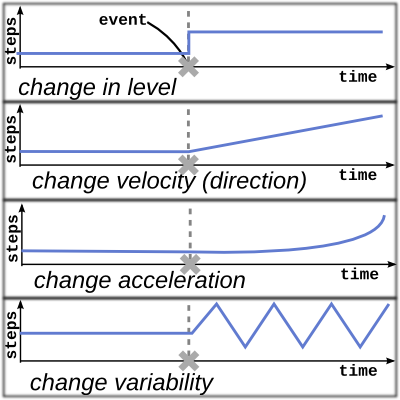
\includegraphics[width=0.6\columnwidth]{./img/exampleDynamicSignals.png}
\caption{Theoretical responses to an intervention (adapted from \cite{glass1975}).}
\label{fig:exampleSignals}
\end{figure}

Figure \ref{fig:exampleSignals} shows the case where an event instantaneously causes permanent change in the target behavior, but in the many cases the intervention will have a temporary effect on the target behavior and will have some delay before setting in.

\begin{figure}
\centering
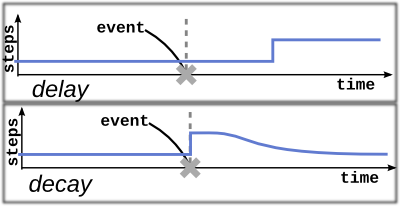
\includegraphics[width=0.6\columnwidth]{./img/exampleDynamicComplications.png}
\caption{Level-change responses with delay and decay (adapted from \cite{glass1975}).}
\label{fig:exampleComplications}
\end{figure}

These intervention response dynamics as shown in figure \ref{fig:exampleComplications} are critically important for just-in-time adaptive intervention developers, but are largely unaddressed in current theory.
One method for examining event dynamics is to explore each particpant's record individually (perhaps segmented by day), and to mark the events and manually explore individual responses.
Since this examination is taking place over many series, it is prudent to utilize sparklines \cite{tufte2006} or horizongraphs \cite{reijner2008} to allow for examination of many series simultaneously.
In doing this, however, it quickly becomes apparent that behavioral intervention data in this format is much too unweildy.
Random contextual fluctuations and inconsistency in frequency of intervention delivery makes visual identification of patterns extremely difficult when viewing an entire series, let alone series for multiple participants. 
Thus, we focus first on the characterizing the response to single events only, and can later address the issue of event history treated as a contextual subgrouping of all events.

\subsection{Event-time Alignment}
Plotting individual events one-by-one allows a researcher to explore the ideographic details of that particular event, but in order to draw out generalizations across groups of events (be it by participant, context, or any other selector) events must be plotted relative to the time of the event, rather than the start of the study.
By time-shifting our data view so that each intervention event falls at t=0 in a time-series, we can view many events on a common time frame.

\begin{figure}
\centering
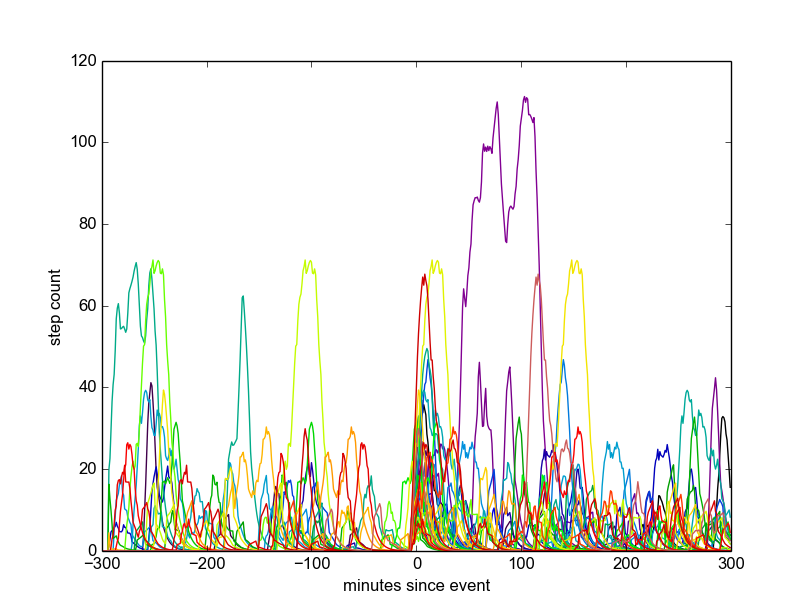
\includegraphics[width=0.9\columnwidth]{./img/perfect_intervention_individual_events_smoothed.png}
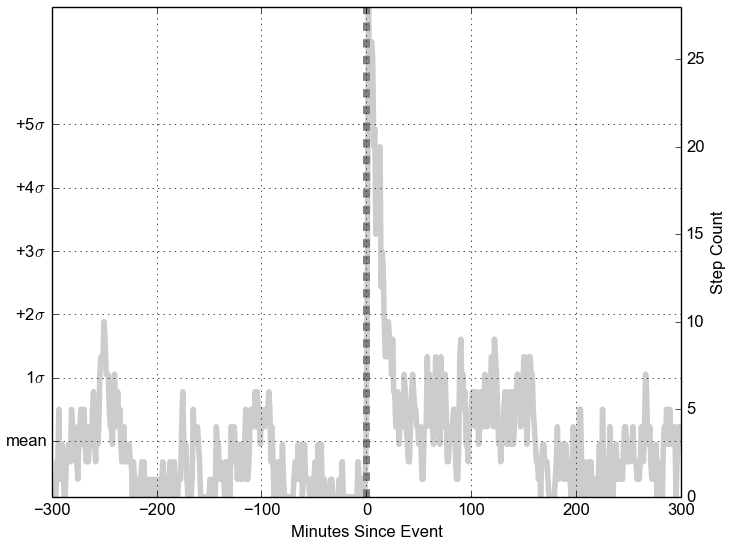
\includegraphics[width=0.9\columnwidth]{./img/perfect_intervention.png}
\caption{Comparison of all event responses smoothed over a 15m rolling window (top) to average response (bottom) surrounding the control dataset intervention.}
\label{fig:interventionAverage}
\end{figure}

Figures \ref{fig:exampleSignals} and \ref{fig:exampleComplications} give us sense of what an intervention should look like, but in reality individual variations in context completely mask the often small effect of an intervention (see Figure \ref{fig:interventionAverage} (top)).
To a researcher looking at the plot of individual event responses figure \ref{fig:interventionAverage} (top), it might seem that only the intervention plotted in purple was an effective intervention, acting with a delay of approximately 30m, and decaying rapidly 120m after the event.
However, we know that the control dataset - by design - includes interventions that were 100\% effective, acting with minimal delay and beginning decay at 5m.
Plotting these series with aforemented ``summary dashboard'' methods may allow researchers to identify this pattern more easily, but the average signal is still difficult to pull out of the noise.
Luckily, this is a familiar problem with a familiar solution.
Since our data has been time-shifted to place the time of event at t=0, we can simply average the series together in order to identify nomothetic trends across all events.
When looking at all events individually (figure \ref{fig:interventionAverage} top), it is difficult to spot any pattern in the series.
When averaging across all event responses, however, a clear, significant response is evident (figure \ref{fig:interventionAverage} bottom), and the purple series is exposed as an outlier.

This approach can be taken for all events in one subject's time series to characterize that subject, or can be applied across subjects to characterize a more generalized response to the intervention.

As expected, figure \ref{fig:interventionAverage} shows the control intervention to be quite effective at increasing the step count.
The additional y-axis showing the mean and standard deviation of the series is included to give an increased sense of the significance of this effect relative to data which may be out of frame.
In addition to the nearly immediate response, a longer-lasting effect reaching out to approximately 180m after the event seems to be boosting step count, though the all-events view in figure \ref{fig:interventionAverage} as well as the stacked-events display in Figure 1 reveal that there are two events which may be the the cause.
Though the average line-graph makes spotting effects easy, we must be wary of outlying events or participants which can skew the average.
This danger can be sometimes mitigated through use of median in place of mean, but since step-count does not obey a normal distribution (0 values are almost always modal), that approach does not work well in this case.

\subsection{Stacking}
To address the shortcomings of the aforementioned average-line shown in figure \ref{fig:interventionAverage}, individual events can be shown on the graph and stacked.
This yields the same shape, and the y-axis can be easily normalized to match our average series by dividing by the number of events.
While still “averaging out” random contextual influences, this visual also provides indication that the average result is not due to one outlier event, enables easy spotting of missing data or faulty sensors, and gives some indication of the number of events considered.
For an n-of-one dataset such as the control dataset, events can be graphed with a unique color.
In figure 1, event colors are chosen based on the order in which they were observed.
Color mapping of events can also be used to visually group events based on time of day, location of the event, or participant.

\begin{figure}
\centering
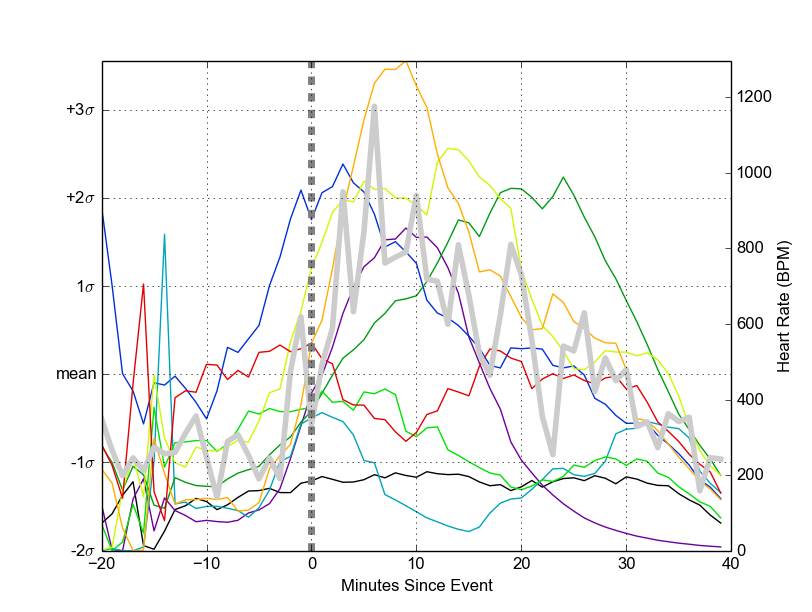
\includegraphics[width=0.9\columnwidth]{./img/knowMe_60m_lines_smoothed15m.png}
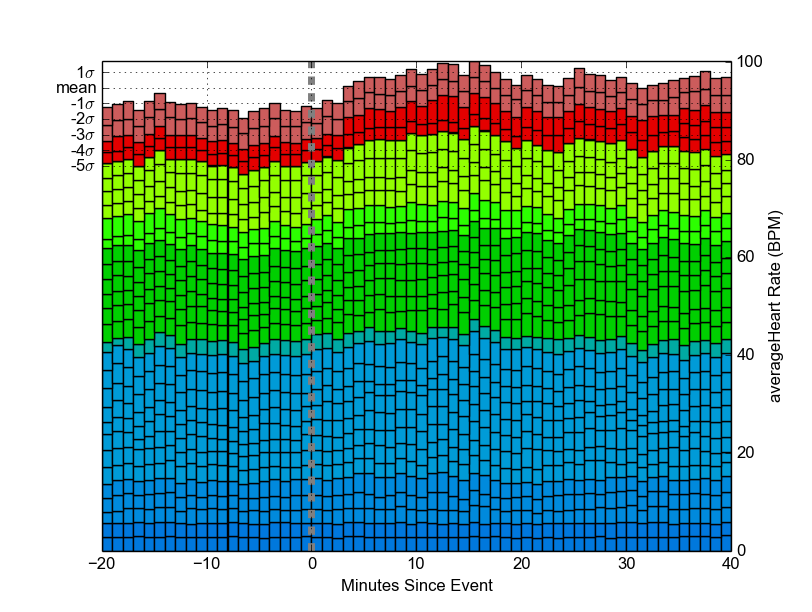
\includegraphics[width=0.9\columnwidth]{./img/knowMe_60m_bars.png}
\caption{Comparison of knowMe average lines (smoothed over 15m rolling window) and stacked bars.}
\label{fig:knowMeCompare}
\end{figure}

Figure \ref{fig:knowMeCompare} shows the difference between a plot of various average response lines and the stacked area plot.
The thin lines in figure \ref{fig:knowMeCompare} (top) represent the response of each participant to the event averaged across all events for that participant.
The thick line shows the average across all participant’s average series.

The stacked bars in figure \ref{fig:knowMeCompare} (bottom) are colored by participant ID, and each represent one unique event - stacked in order of event incidence.
This allows researchers to search for both participant outliers within the set as well as event outliers within each participant.
The deviation from the mean as measured relative to the standard deviation gives a sense of how unlikely the signal is to be a random artifact, but methods for evaluating the statistical likelihood of observing a particular shape are not covered here.
Figure \ref{fig:knowMeCompare} shows an increase in heart rate following the delivery of a physical-activity-suggesting sms message.
Though the behavioral measure differs greatly from that used in the control dataset and \ref{fig:interventionAverage}, a comparison of the y-values in terms of standard deviation also reveals that this effect is less extreme than what we observe in the control intervention.
For additional comparison to the control data, also consider the average-line view in figure \ref{fig:interventionAverage}, and the stackplot shown in figure 1B.
Though the highlighted windows are relatively small (to highlight the intervention response), much wider context around the event can be plotted, such as that shown in figure 1A.

This same analysis is applied to figure 1C, and the correlation between the increase in acceleromtry counts and heart rate is clear.
Note however, the different dynamics of each variable's response.
Accelerometry counts are more directly tied to behavior, and thus the dyanamics observed are more volatile, while heart rate acts as smoothed function of accelerometry, responding less quickly and decaying more slowly than accelerometry data.

The linegraph allows for characterization of unqiue individuals, but the stackplot better highlights the overall effect and also shows the number of events considered.
Another key difference between these two approaches is the proporitonate weighting of subjects into the global effect display.
The line-graph approach considers each subject equally regarless of the number of events recorded of that subject, whereas the stackplot considers the events equally and thus each subject's contribution is weighted by the number of events recorded.

\begin{equation}
	\bar{y}(t) = \frac{1}{N} \sum\limits_{i=1}^N y_i(t)
	\label{eq:barAvg}
\end{equation}

\begin{equation}
	\bar{y}(t) = \frac{1}{P} \sum\limits_{p=1}^P \frac{1}{n_p} \sum\limits{i=1}^n_p y_{i,p}(t)
	\label{eq:lineAvg}
\end{equation}
	
Equations (\ref{eq:barAvg}) and (\ref{eq:lineAvg}) shows the difference in aggregation methods for line vs stacked views where $N$ is the total number of events across all participants, $P$ is the number of participants, $n_p$ represents the number of events for subject $p$,  $y_i$ represents the time series for event $i$, and $y_{i,p}$ represents the time series for subject $p$'s event $i$.
Aggretating data via method (\ref{eq:lineAvg}) does a better job to ensure that one participant does not skew results, but can give too much weight to data from a participant with few events.

\subsection{Characterize Intervention Delivery Context}
In some cases introducing a “control event” against which to compare the experimental event can help isolate the intervention from the context in which it is delivered.
For instance, an intervention delivered on a mobile device is always delivered within the context of phone interaction.
That is, the user is always using the phone when the intervention is delivered.
It is possible that "using the phone" has it's own unique effect on the behavioral measure.
Thus, using "phone use" events as a baseline against which to compare "phone use and intervention delivery" strengthens the chance that the observed effect is a result of the intervention itself and not the result of frequently concurrent contextual forces. 
For example, by looking at all times the phone was viewed in the mAvatar dataset, we can characterize the average context of phone use.

\begin{figure}
\centering
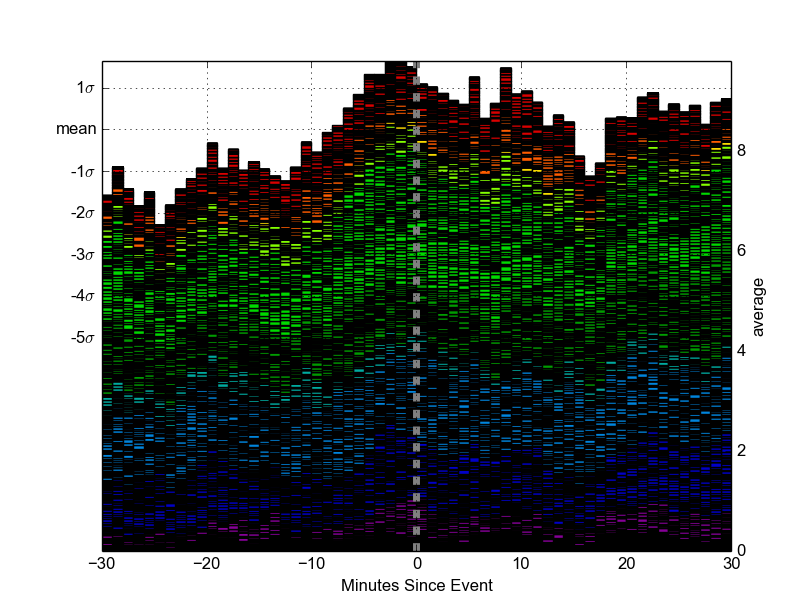
\includegraphics[width=0.9\columnwidth]{./img/mAvatarViews_1673_wOverlap.png}
\caption{Stackplot of step counts in the 30 minutes surrounding 1673 phone-view events from the mAvatar dataset.}
\label{fig:mAvatarPhoneContext}
\end{figure}

In figure \ref{fig:mAvatarPhoneContext}, we see a notable increase in steps leading up to phone usage.
It is possible that this increase - though it prempts avatar viewing - is indeed caused by the avatar.
Consider, for instance, the unanimously reported case of subjects viewing the phone with the explicit purpose of seeing how the avatar would be affected by their behavior.
Thus we should perhaps expect to see a peak in PA driven by the desire to illicit a response from the avatar, which is viewed only a few minutes later.
This interpretation is quite speculative and other features of figure \ref{fig:mAvatarPhoneContext} are not so easily explained.
It is clear, however, that this is not a flat baseline that we may expect to find on average, and exploration of dynamics surrounding the active and sedentary avatar viewings ought to subtract this baseline to account for the overlapping of this context-driven (rather than event-driven) signal.
This masking baseline signal is apparent in the unadjusted plot of active-avatar views shown in figure 1D. 
Rather than a comparison of each event vs the baseline, however, the specific case of the mAvatar dataset allows us to utilize a direct comparison between similar, opposing events (active-avatar vs sedentar-avatar).

\comment{
The results of this analysis were not interesting; the control data looks the same when processed this way

Using the control dataset as an example, random points in time when the subject was at his desk can serve as the control event against which to compare the experimental "intervention" event.

To represent a difference between two intervention effect time series visually we return to the use of line averages due to the confounding nature of negatively-valued bars in stacked graphs.

TODO: fig line graph of controlData avg(intervention)-avg(control)
}

\subsection{Comparing Event Types}
Aforementioned methods used to provide a contextual baseline of comparison for events can also be applied to allow for a comparison between two event types.
By treating one event as the baseline, differences between the events can be visualized.
Using this paradigm, nearly equivalent event responses will have a near-zero difference.
Positively-valued areas of the resulting chart indicate times when the "experimental event" had a greater positive effect on the target measure, or, conversely, that the "control event" had a greater negative effect on the target measure.


The mAvatar dataset contains two types of intervention which may be interesting to compare: 1) active-avatar viewing, 2) sedentary-avatar viewing.
In this case, the two event types are theoretically opposite in effect, meaning that the sedentary-avatar effect should resemble a mirrored version of the active-avatar effect.
Thus, the difference should accentuate the intervention's effect signature and better isolate the behavioral response from noisy data.

\begin{figure}
\centering
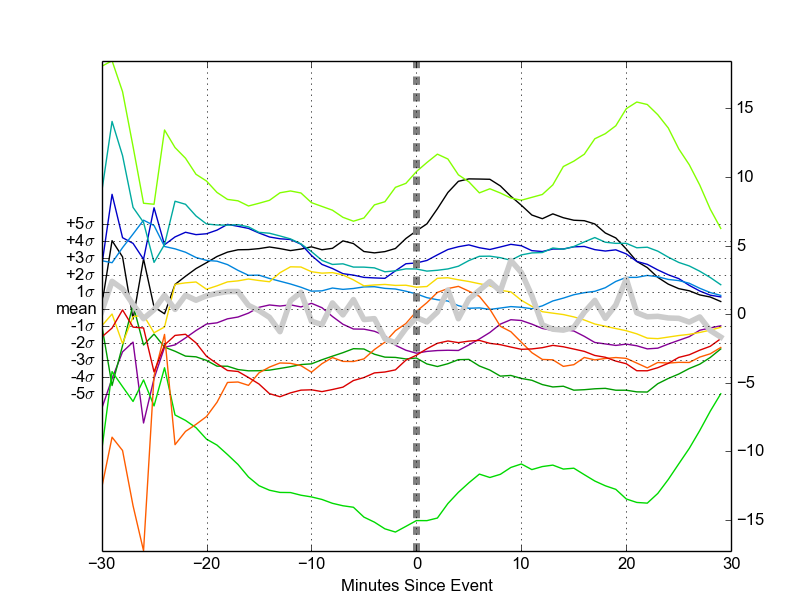
\includegraphics[width=0.9\columnwidth]{./img/mAvatar_difference_events_smooth15m.png}
\caption{Active-event series average minus sedentary-event series average smoothed over a 15m rolling window. (average across participants shown in bold)}
\label{fig:mAvatarDifference}
\end{figure}

Even with two oppositely-polarized events figure \ref{fig:mAvatarDifference} fails to show the dramatic effect a researcher might hope for on average.
The lack of observed effect indicates that the intervention had no effect on average.
In this case, researchers attribute the apparent lack of effect to an ambiguity in study design which led to two opposing conditions: 1) subjects respond positively to physically-active avatars via the Proteus Effect \cite{yee2009proteus} 2) subjects respond negatively to physically-active avatars via falsely perceived biofeedback.

Figure \ref{fig:mAvatarDifference} suggests this subgrouping within the data in the individual participant series.

TODO: talk more about the subgroups (+ response vs -response), label the series.

\comment{
\section{Domain Expert Feedback}
TODO: what do domain experts think about these methods (Donna? Eric?)
}

\section{Discussion and Future Work}
Though the presented work helps address some of the challenges faced by contemporary behavioral researchers, in some places there remains uncertainty in the meaning of the visualizations and even more deeply hidden discoveries.
Additionally, new scientific questions have been raised through application of these visualizations and thus future work is required.


\subsection{Dealing With Overlapped Data Frames}
When looking at data surrounding an event, we must be cognizant of how instances of the same event at another time may effect our data.
For instance, if our analysis targets the 30m following an event, and the event frequently occurs at 10m intervals, the overlapping signals will create unwanted artifacts.

\begin{figure}
\centering
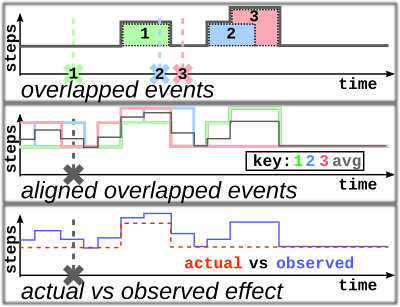
\includegraphics[width=0.6\columnwidth]{./img/eventOverlapExample.png}
\caption{Overlapping analysis windows confounds observed effect after time-alignment.}
\label{fig:overlapExample}
\end{figure}

Figure \ref{fig:overlapExample} illustrates this point by showing how events falling within each other's windows of analysis confound the data and ultimately yields a signal quite unlike the actual effect response.
In real data, this is further complicated by the non-linear way in which effects are expected to combine.
An example of this effect in real data can be seen in the four yellow to lime green series plotted in figure \ref{fig:interventionAverage} (top).
The yellow peak near 0m represents a true intervention response, whereas the other three are artifacts introduced from relative nearness in time to the true response.
In other words, the events analyzed in each of these series fall at approximately -280, -150, 0, and 120 minutes relative to the third event, and those artifacts all represent the same data.
Study designs utilizing methods outlined in this paper should design studies to minimize overlapping analysis windows.

\begin{figure}
\centering
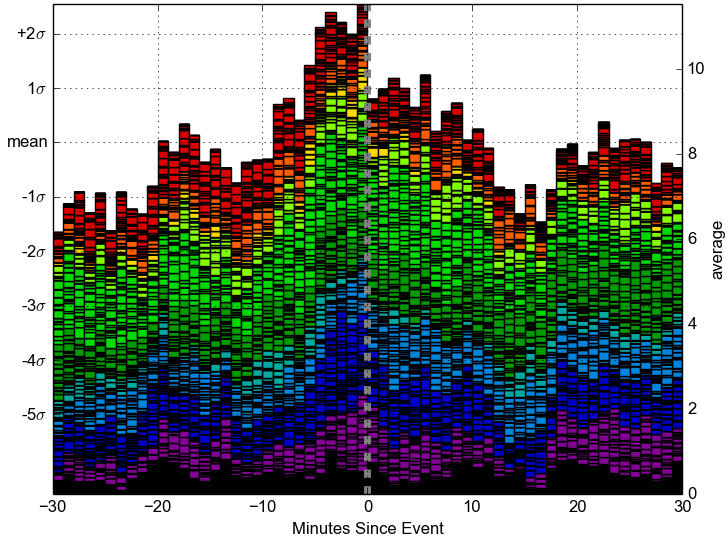
\includegraphics[width=0.9\columnwidth]{./img/mAvatarViews_586_noOverlap.png}
\caption{Stackplot of step counts in the 30 minutes surrounding 586 phone-view events from the mAvatar dataset with no other events within 30min.}
\label{fig:mAvatarNoOverlap}
\end{figure}

Event overlap becomes somewhat inevitable, however, for large event window sizes.
Figure \ref{fig:mAvatarNoOverlap} shows a selection of data identical to that in figure \ref{fig:mAvatarPhoneContext}, but without the inclusion of overlapping windows of analysis surrounding the events.
Allowing no overlap between events helps ensure that multiple interventions effects do not skew the data, but ignoring these data points can drastically reduce the sample if large times following the event are used, because very few events are so isolated.

\begin{figure}
\centering
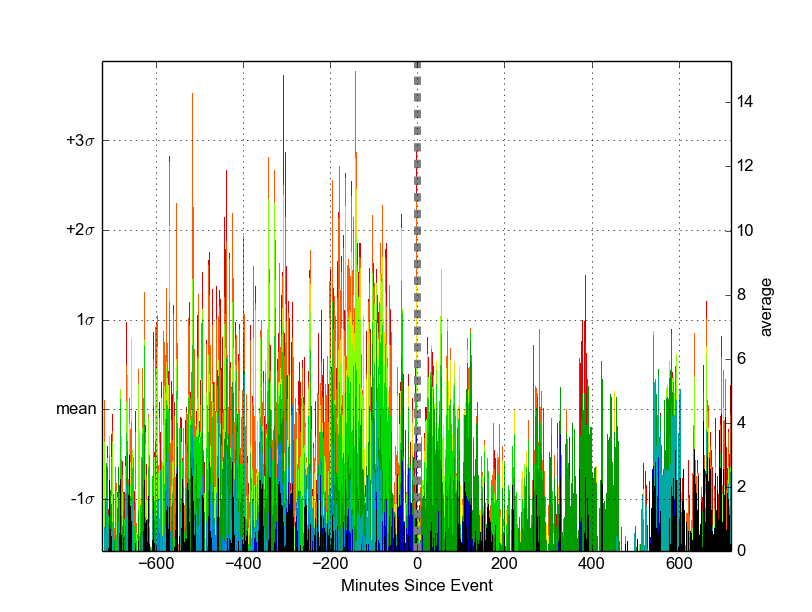
\includegraphics[width=0.9\columnwidth]{./img/mAvatarViews_46_12hr_noOverlap.png}
\caption{Stackplot of step counts in the 12hrs surrounding 46 phone-view events from the mAvatar dataset with no other events within 12 hours.}
\label{fig:mAvatarNoOverlap12hr}
\end{figure}

As is shown in \ref{fig:mAvatarNoOverlap12hr}, increasing the window of analysis to 12hours surrounding the phone-view event leaves only 46 events, and a noticeable increase in the variability of the data is observed.

\begin{figure}
\centering
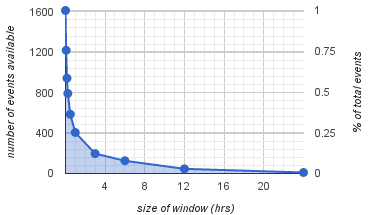
\includegraphics[width=0.9\columnwidth]{./img/events_v_windowSize.png}
\caption{Percent coverage of events in the mAvatar datset vs size of exclusion window surrounding the event.}
\label{fig:eventsVwindow}
\end{figure}

For phone-view events among the population analyzed by the mAvatar study, we can estimate percent coverage of events available for ``clean'', non-overlapping analysis through the distribution shown in figure \ref{fig:eventsVwindow}.

\subsection{Alternative Stacked-Area Representation}
Use of the "themeRiver/streamgraph" \cite{havre2000, byron2008} paradigm for plotting stacked area charts may offer an improved view of the contribution of individual time series to the aggregated result, further easing the identification of outlier participants or events.

With better focus on individuals or subgroups, however, comes a reduced ability to look at the bigger picture.
Thus, although a streamgraph may make for a better general view, the stacked area plots presented are still of use for those whose primary focus it is to evaluate the group response.

\comment{ things covered by this section are well discussed elsewhere
  \subsection{Modeling Observed Effects}
  Ever since [], behavioral scientists have sought theories to explain, influence and change human behavior.


  TODO? Some example models of the aforementioned effects for control and/or KNOWME data.

  transfer function modeling?
  fitting of a fluid-flow analogy using a priori constructs?
  other?
}

\subsection{Characterizing Psychological Influence of Events via Response Signature}
Different psychological mechanisms act on different time-scales and, likewise, with different dynamics. 
The delay of effect onset and decay of the effect observed in data could theoretically be used to suggest what psychological mechanisms are at work.
In this way, interventions could be characterized in terms of applicable theory via the the dynamics observed.

This method becomes even more powerful when responses across multiple variables are considered.
To draw an example from previously presented data, a combined analysis of heart rate (figure 1C) and accelerometer count (figure \ref{fig:knowMeCompare}) dynamics improves the ability to match signals to known responses.

\subsection{Statistical Analysis of Features}
Much existing work on the statistical testing of between-phase differences in traditional AB study designs \cite{parker2003} is applied in the evaluation of the efficacy of a one-time or repeatedly applied intervention, and methods for evaluating the likelihood of features in a time-series are also well documented \cite{gorman1996, suen1989}.
Through combination of existing intervention analysis techniques \cite{box1975}, goodness-of-fit evaluations of model formulations \cite{pankratz2012} in comparison to surrogate time series, and the presented visualization methods, researchers have a good foundation for analyzing dynamic models of human behaviors. % to enable clever JiTAIs.

\section{Conclusion}
There are many reasons why behavior change is hard: people build up habits over time, behaviors may be tied to addictive substances or activities, behavior is tied to normal daily human experience and context (i.e. smoking more often when with a certain group of individuals or in a particular location).
The full potential of behavioral interventions - particularly JITAIs - will continue unrealized until mechanistic methods of behavior modeling are adopted by the behavior science community.

The presented visualization methods allow for more detailed analysis of how a subject’s behavior responds to a stimuli over time.
These methods, when combined with a computational modeling approach to understanding human behavior may enable behavioral scientists to formulate more accurate and more application-ready theories, leading to more effective behavioral interventions.



 
%% if specified like this the section will be committed in review mode
\comment{
\acknowledgments{
The authors wish to thank A, B, C. This work was supported in part by
a grant from XYZ.}
}

\bibliographystyle{abbrv}
%%use following if all content of bibtex file should be shown
%\nocite{*}
\bibliography{template}
\end{document}
